\begin{columns}

	\column{0.5}
		
	\block{Scientific context \textnormal{\large- Create real-time digital twins of an organ (e.g. liver)}}{
		\textbf{Current Objective :} Develop hybrid \textbf{\fcolorbox{color1!50}{color1}{finite element}} / \textbf{\fcolorbox{color1!50}{color1}{neural network}} methods.
		
		\vspace{-5pt}
		\hspace{495pt} \begin{minipage}{0.5\linewidth}
			\textbf{\textcolor{color2}{accurate}}
			\hspace{25pt}
			\textbf{\textcolor{color2}{quick + parameterized}}
		\end{minipage}
		
		\vspace{15pt}
		
		\begin{center}
			\begin{minipage}{\linewidth}
				\centering
				\begin{tcolorbox}[
					colback=color1!50, % Couleur de fond de la boîte
					colframe=color2, % Couleur du cadre de la boîte
					arc=2mm, % Rayon de l'arrondi des coins
					boxrule=2pt, % Épaisseur du cadre de la boîte
					breakable, enhanced jigsaw,
					width=\linewidth
					]
					\textbf{OFFLINE}
					
					\begin{center}
						\begin{tikzpicture}
							\node at (0,4.0) {Several Geometries};
							\node[draw=none, inner sep=0pt] at (0,0) {
\includegraphics[width=8cm]{images/intro/objective_geom.png}};
							\node[color2,font=\Large] at (5.5,0.3) {+};
							\node at (13,2.6) {Several Forces};
							\node[draw=none, inner sep=0pt] at (13,0) {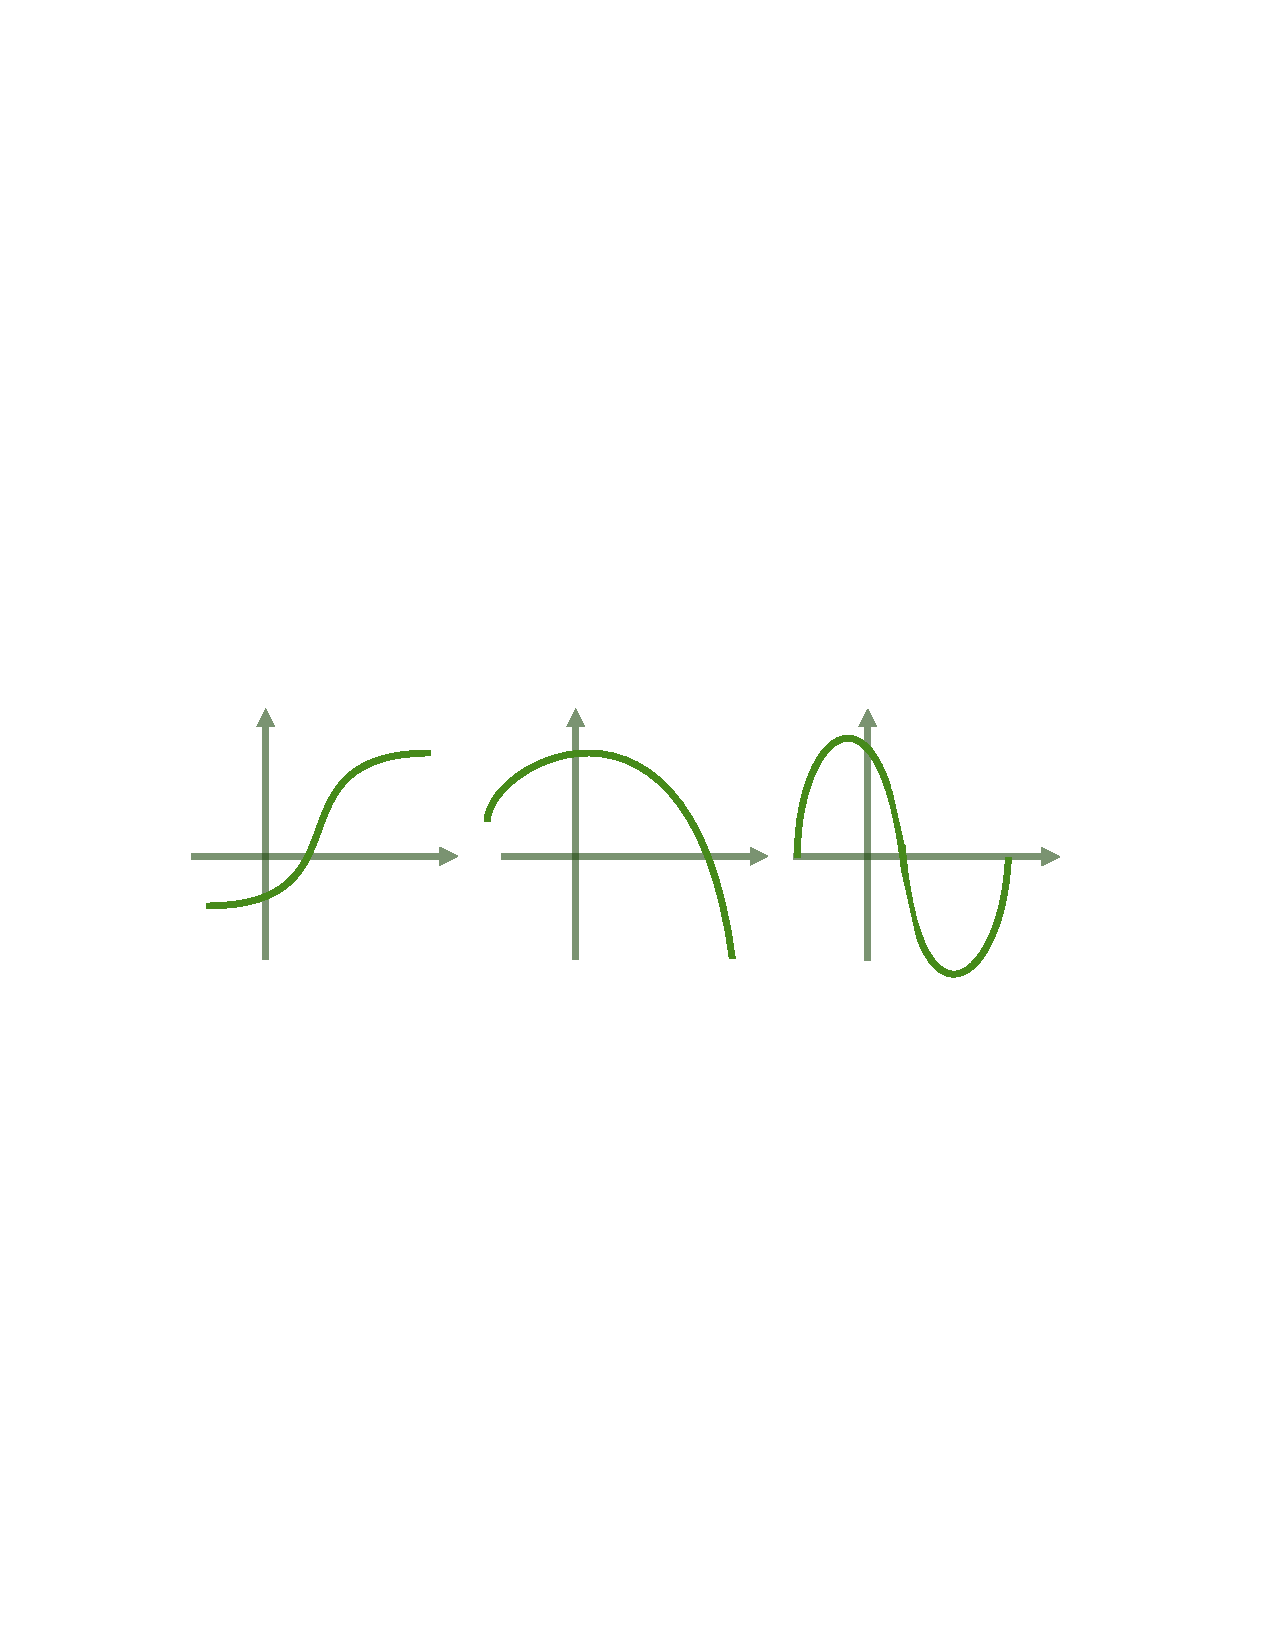
\includegraphics[width=12cm]{images/intro/objective_fct.pdf}};
							
							% Ajouter une flèche entre les deux rectangles
							\draw[->, color2, line width=4.5pt] (20.5,0.3) -- (23.5,0.3);
							%		
							\node at (28,4) {Train a PINNs \textcolor{red}{CITE}};
							\node[draw=none, inner sep=0pt] at (28,0) {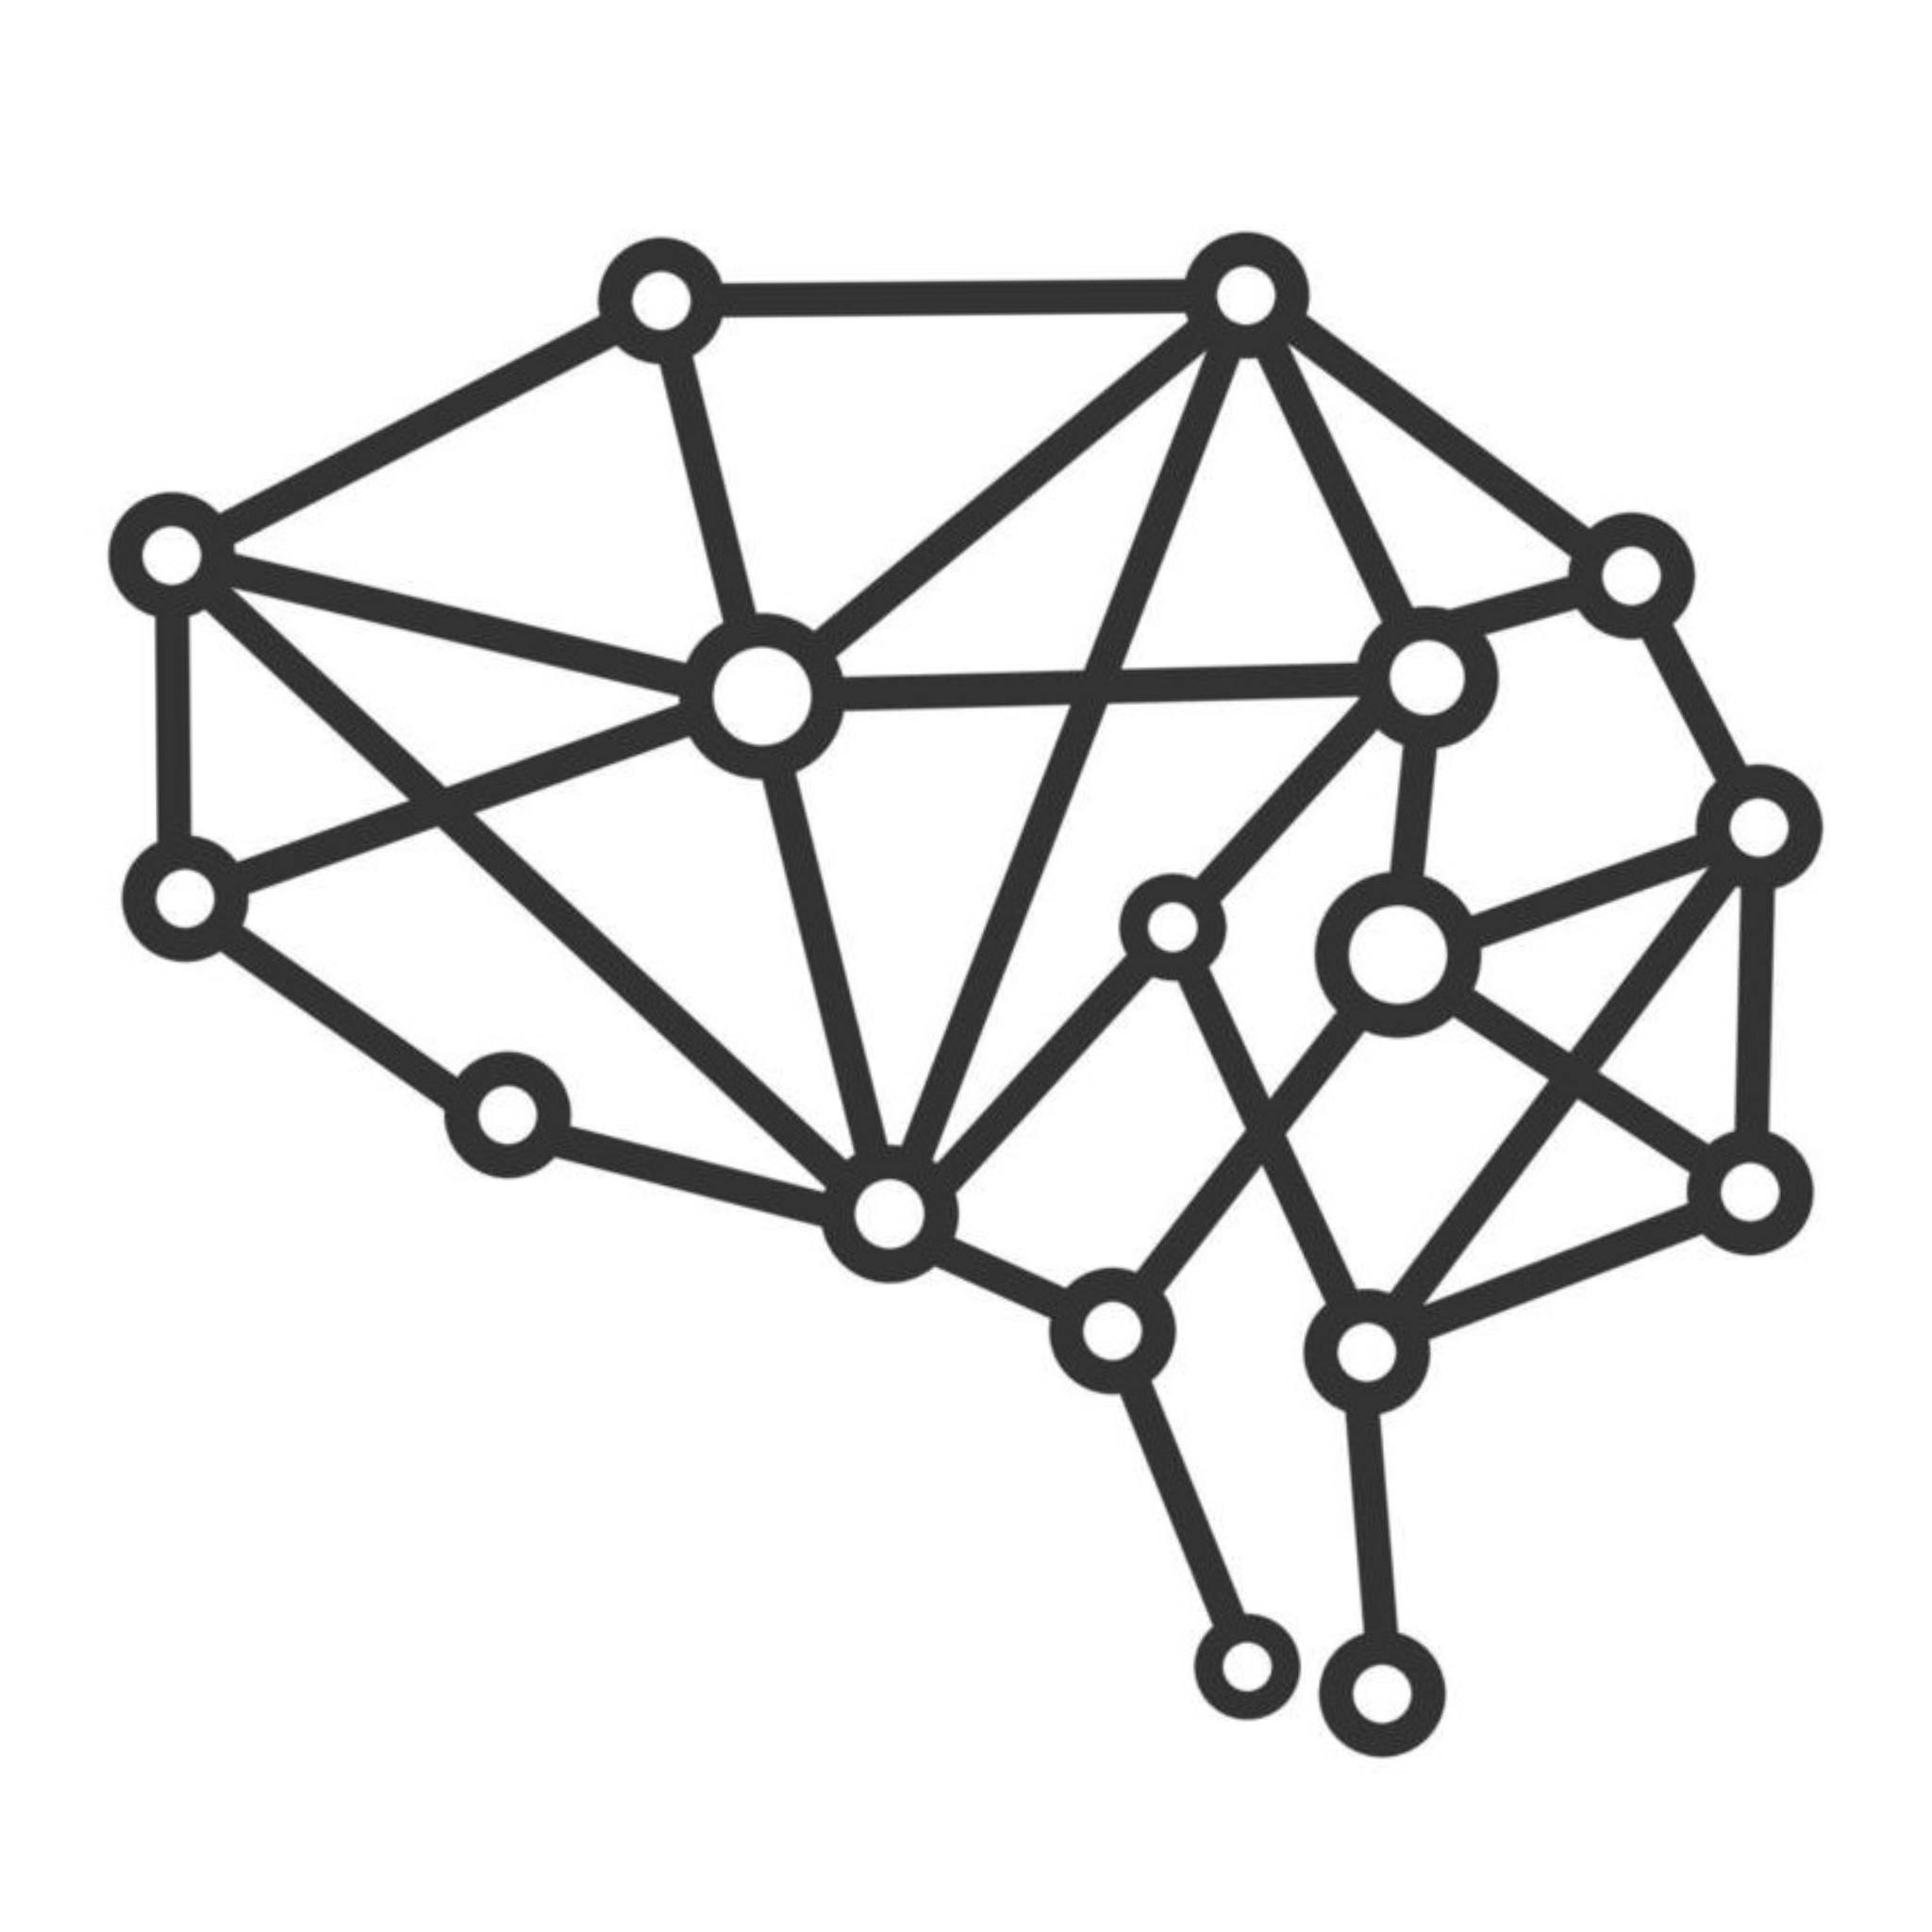
\includegraphics[width=7cm]{images/intro/objective_pinns.png}};				
						\end{tikzpicture}
					\end{center}
				\end{tcolorbox}
			\end{minipage}	

			\vspace{15pt}

			\begin{minipage}{\linewidth}
				\centering
				\begin{tcolorbox}[
					colback=color1!50, % Couleur de fond de la boîte
					colframe=color2, % Couleur du cadre de la boîte
					arc=2mm, % Rayon de l'arrondi des coins
					boxrule=2pt, % Épaisseur du cadre de la boîte
					breakable, enhanced jigsaw,
					width=\linewidth
					]
					\textbf{ONLINE}
					
					\vspace{-10pt}
					\begin{center}
						\begin{tikzpicture}
							\node at (0,2.6) {1 Geometry - 1 Force};
							\node[draw=none, inner sep=0pt] at (0,0) {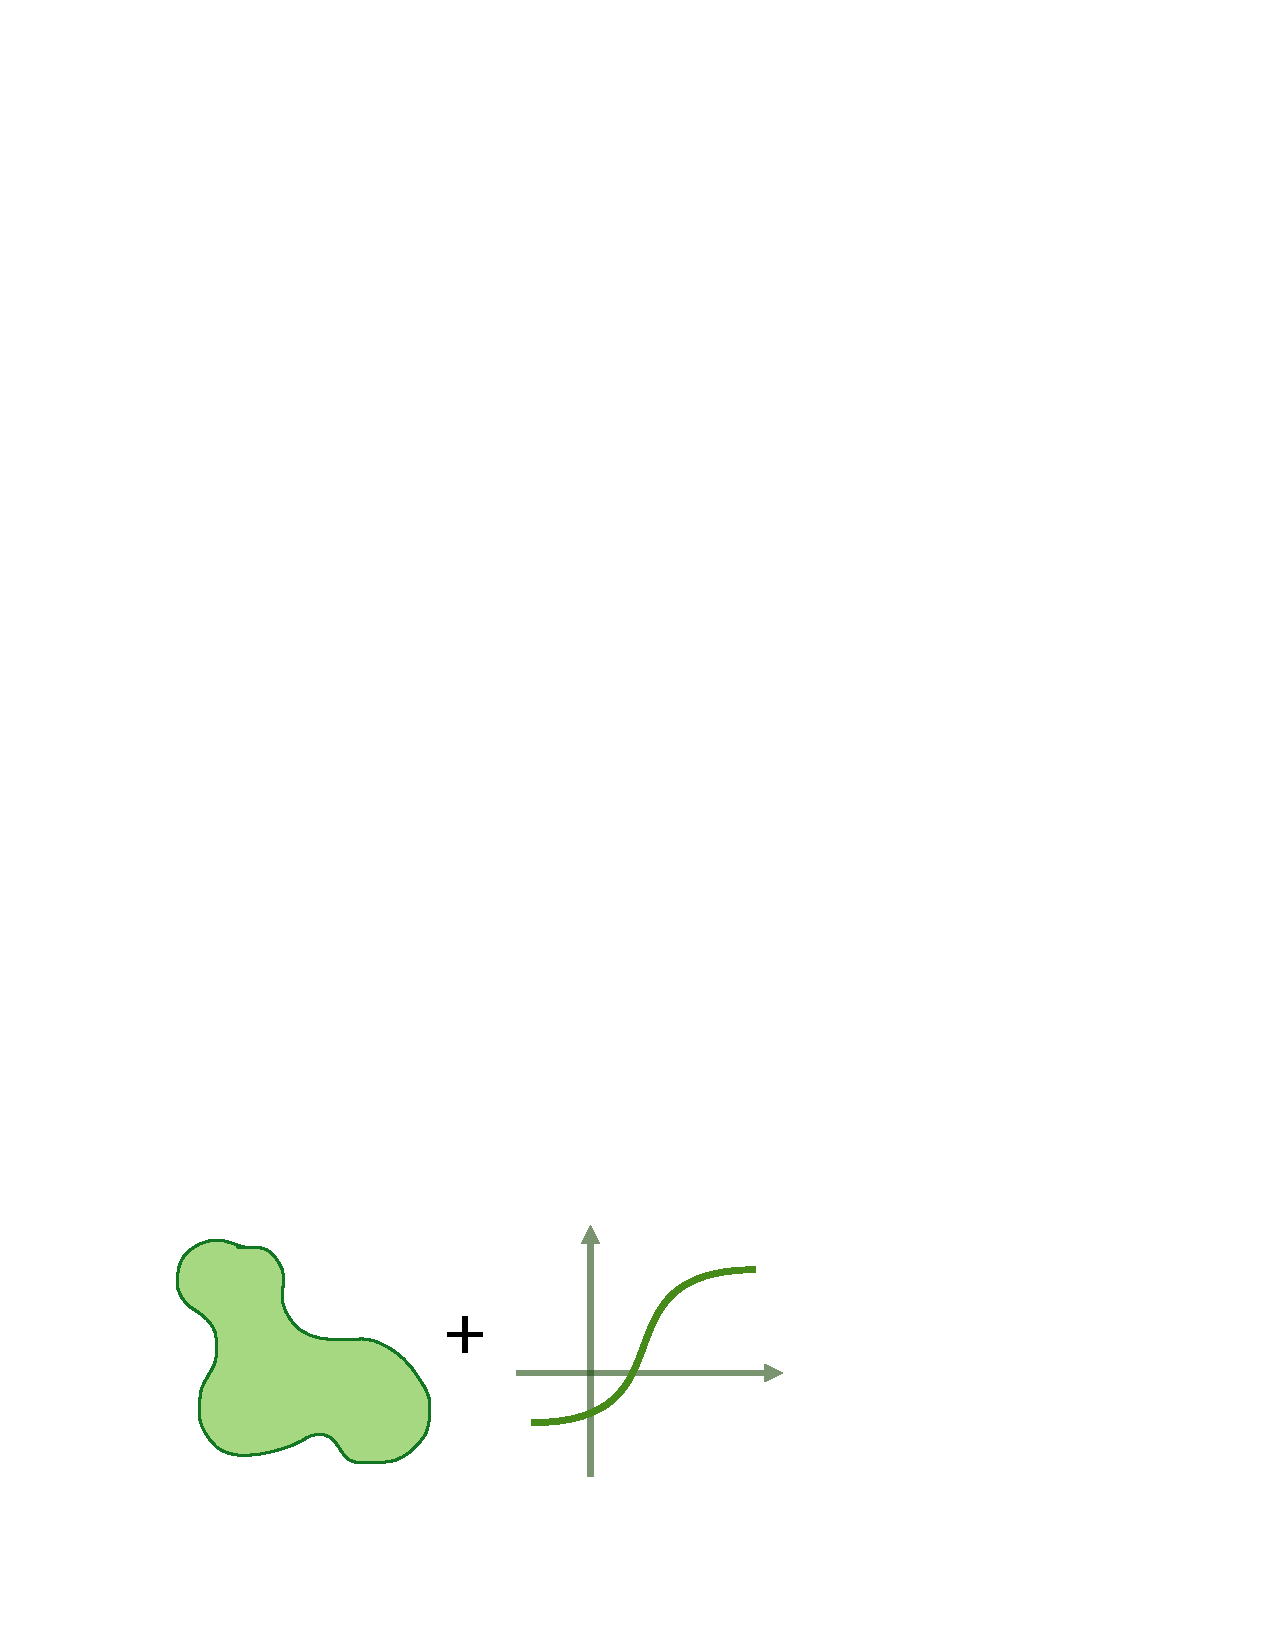
\includegraphics[width=9cm]{images/intro/objective_onegeom_onefct.pdf}};
							%		\node[color2,font=\Large] at (1.6,0.1) {+};
							%		\node at (3.5,0.8) {Several Functions};
							%		\node[draw=none, inner sep=0pt] at (3.5,0) {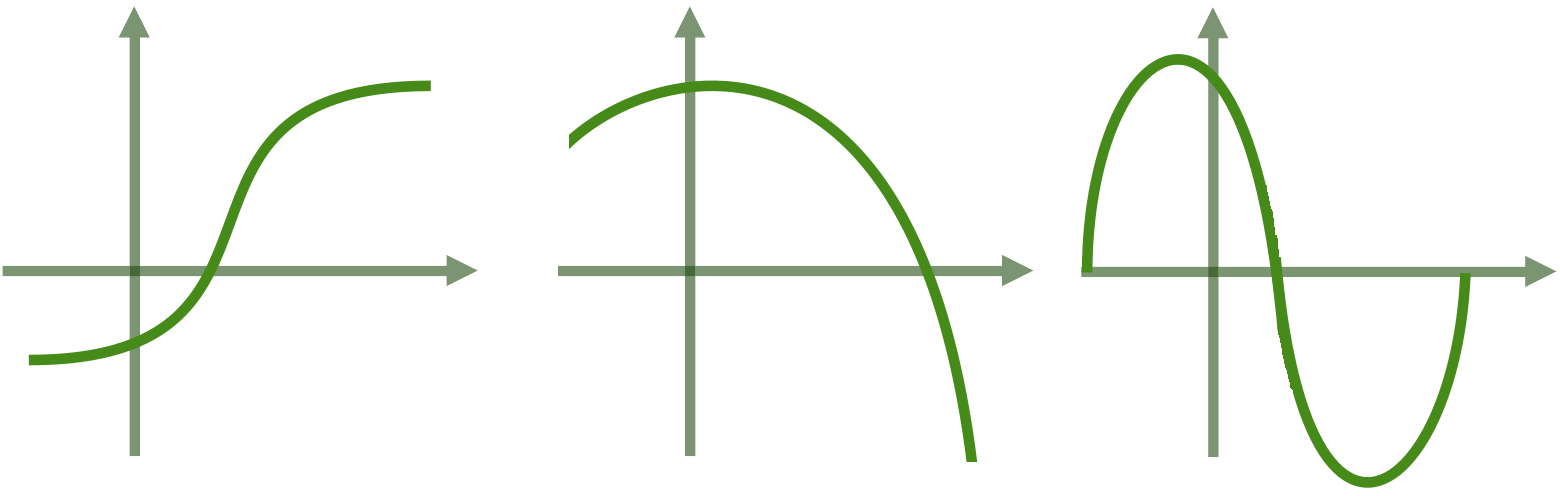
\includegraphics[width=3cm]{images/intro/objective_fct.png}};
							
							\draw[->, color2, line width=4.5pt] (6,0.3) -- (9,0.3);
							
							\node[align=center] at (13,4) {Get PINNs \\ prediction};
							\node[draw=none, inner sep=0pt] at (13,-0.3) {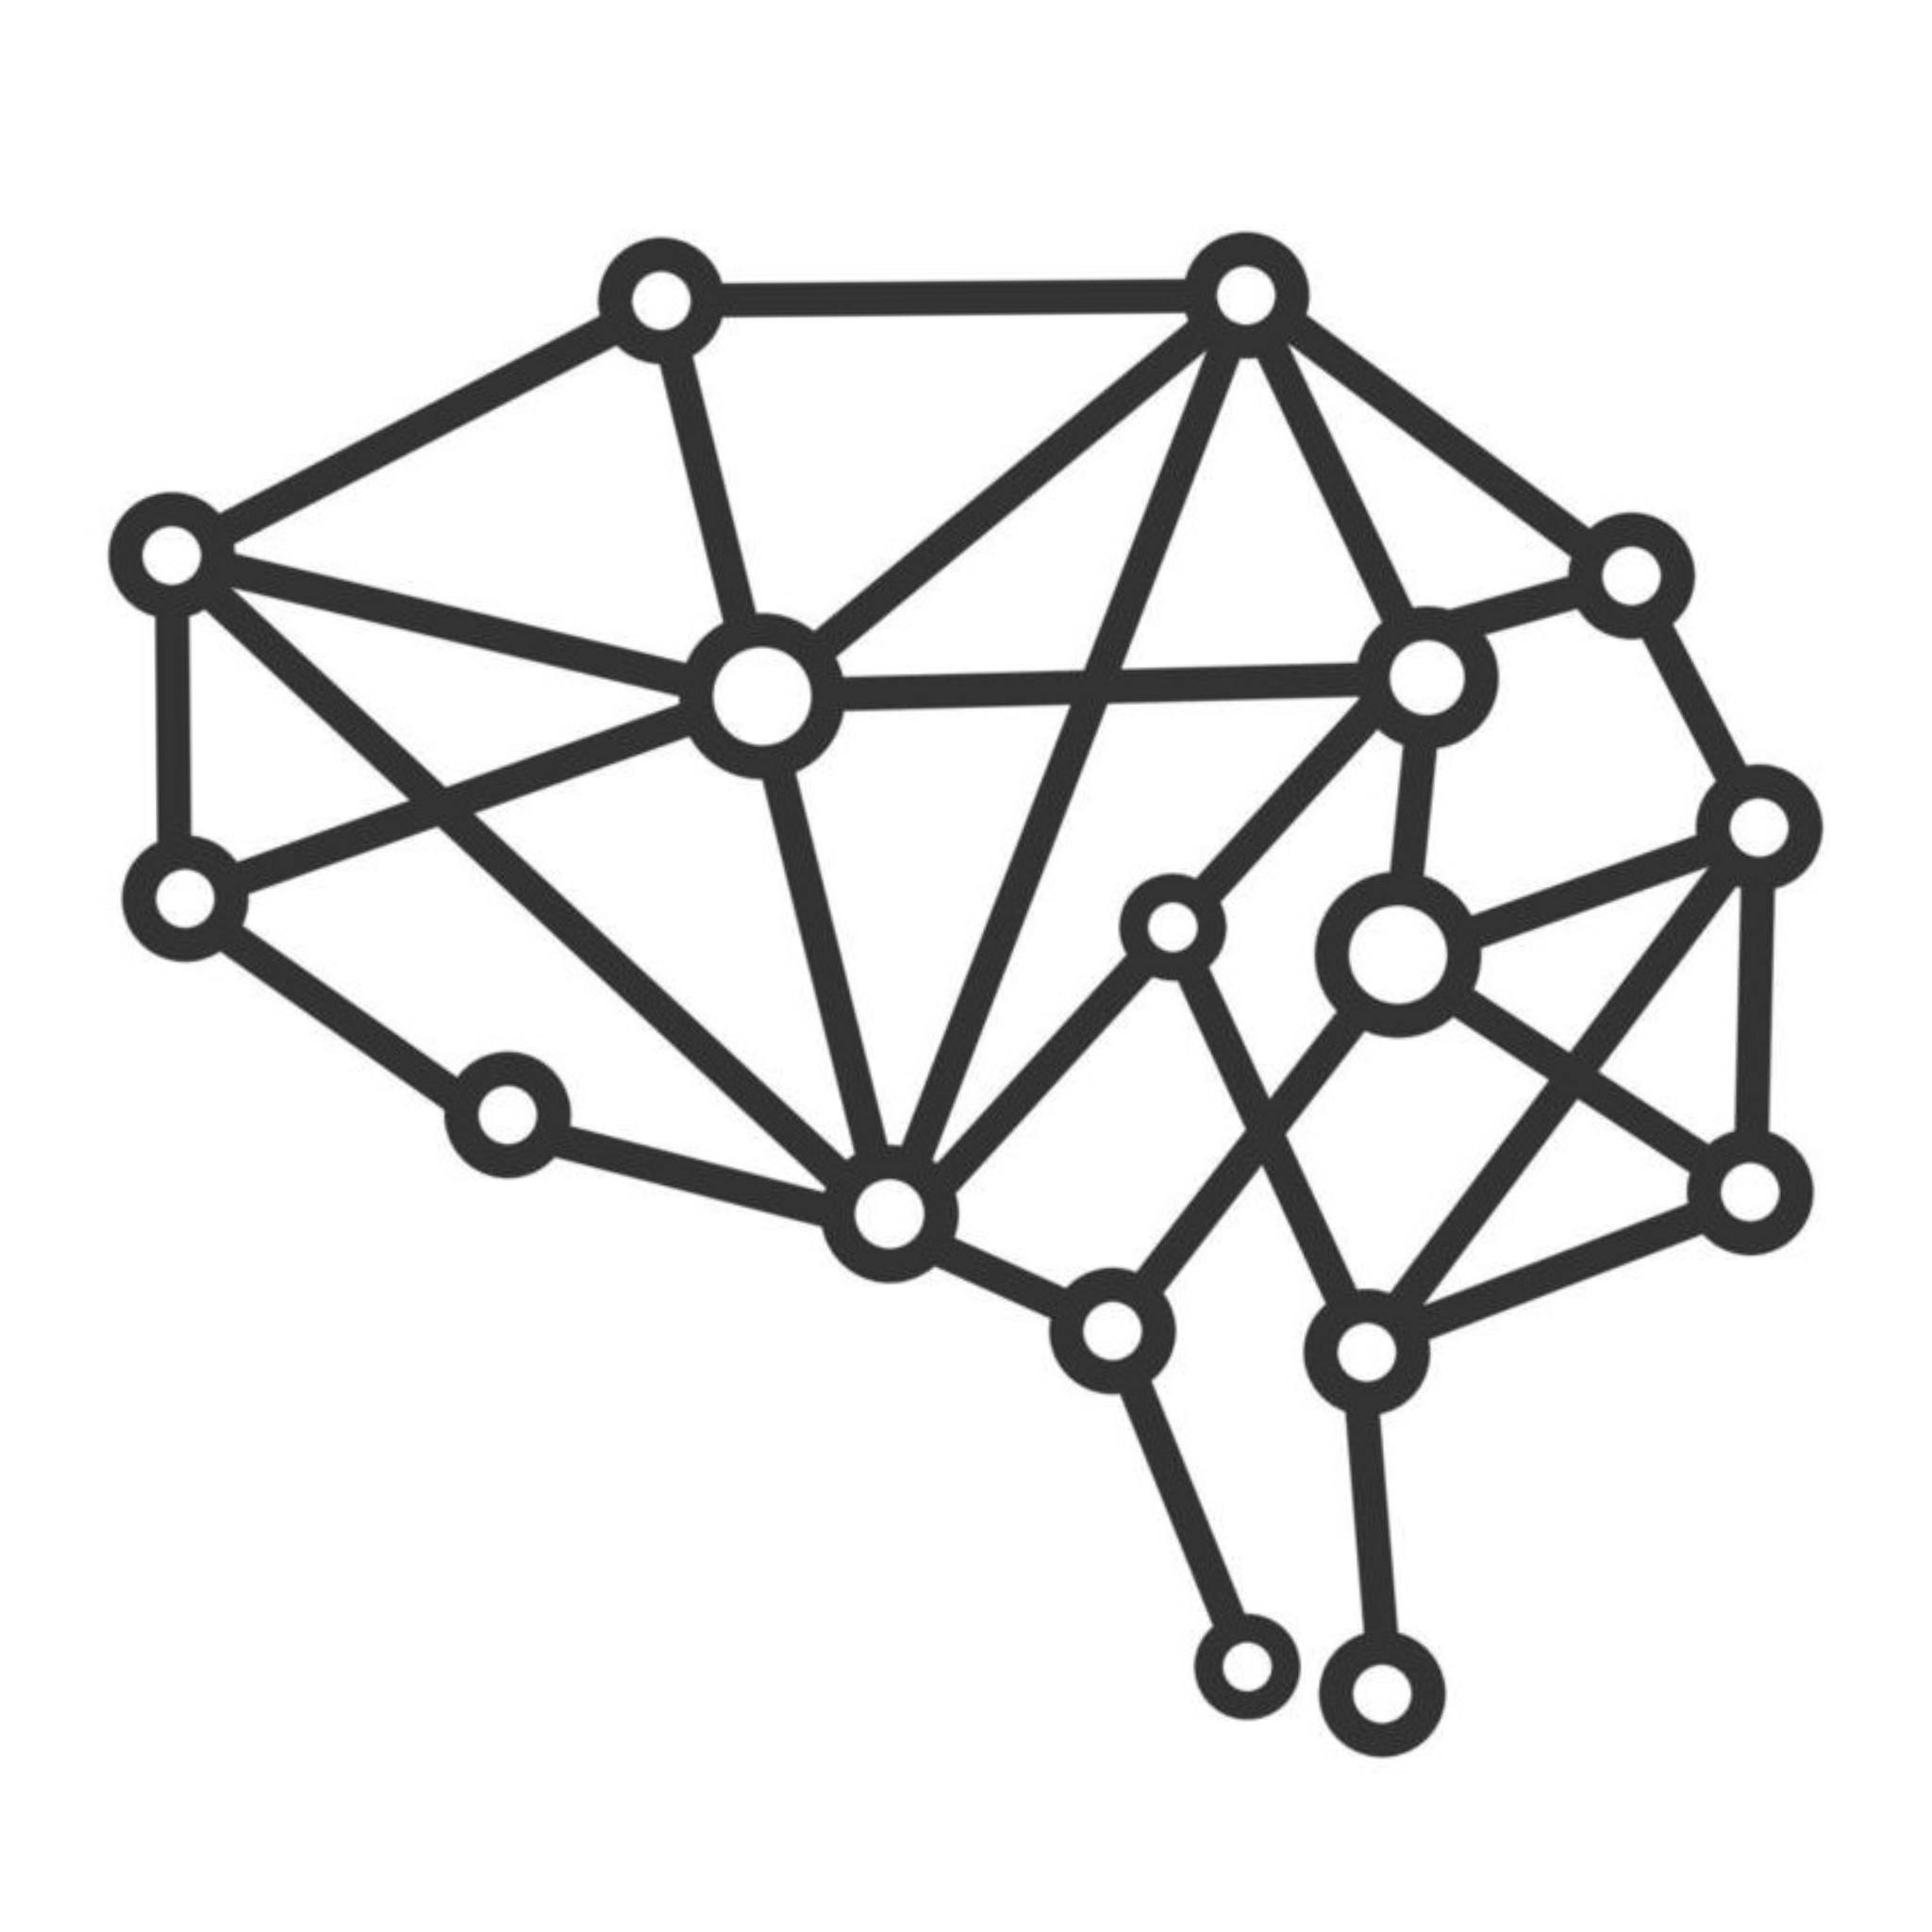
\includegraphics[width=6.5cm]{images/intro/objective_pinns.png}};
							
							% Ajouter une flèche entre les deux rectangles
							\draw[->, color2, line width=4.5pt] (17,0.3) -- (20,0.3);
							\draw[draw=black] (21,-3) rectangle ++(10,8.5);	
							\node[align=center] at (26,4) {Correct prediction \\ with FEM};
							\node[draw=none, inner sep=0pt] at (26,-0.3) {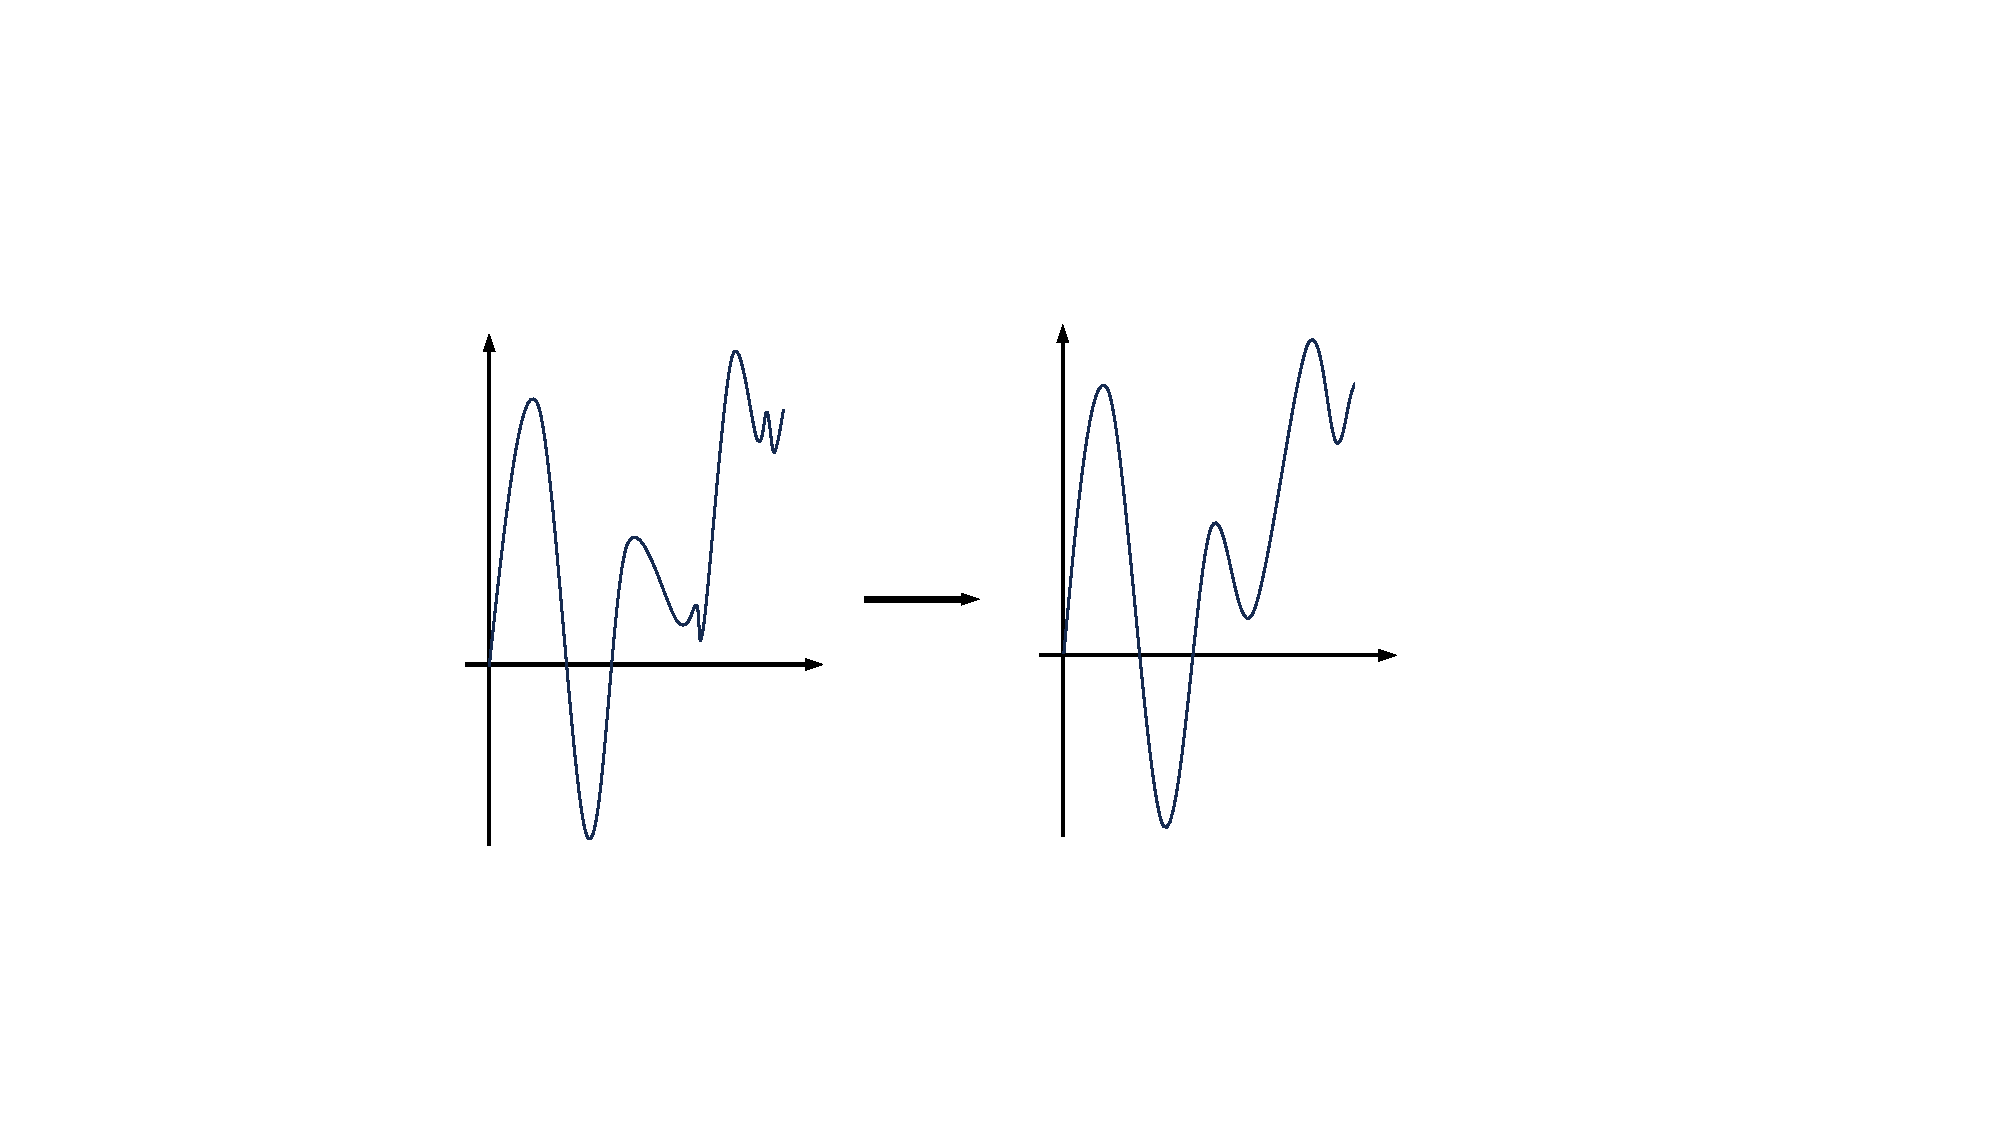
\includegraphics[width=8.5cm]{images/intro/objective_corr.pdf}};		
						\end{tikzpicture}
					\end{center}
				\end{tcolorbox}
			\end{minipage}
		\end{center}		
	}

	\block{Poisson problem with Dirichlet boundary conditions}{
		Find $u : \Omega \rightarrow \mathbb{R}^d (d=1,2,3)$ such that
		\begin{equation}
			\left\{\begin{aligned}
				&-\Delta u(x) = f(x) \quad \text{in } \Omega, \\
				&u(x) = g(x) \quad \text{on } \Gamma
			\end{aligned}\right. \label{edp} \tag{$\mathcal{P}$}
		\end{equation}
		with $\Delta$ the Laplace operator, $\Omega$ a smooth bounded open set and $\Gamma$ its boundary.
	}

	\column{0.5}

	\block{PINNs \textnormal{\large - Physics-Informed Neural Networks}}{
		TODO ?
	}

	\block{Finite Element methods}{
		TODO ?
	}

\end{columns}
